\begin{figure}[h!]
    \centering
    \caption{Distribution of statutory minimum wage changes, Zillow sample}
    \label{fig:mw_changes_dist_zillow}

    \begin{subfigure}{.7\textwidth} \centering
        \caption*{Intensity}
        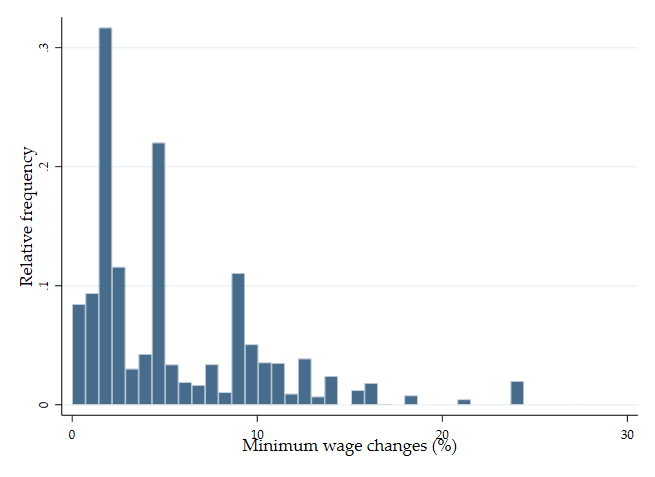
\includegraphics[width = 1\textwidth]
            {estimation_samples/output/pct_ch_mw_dist}
    \end{subfigure}\\
    \begin{subfigure}{.7\textwidth} \centering
        \caption*{Timing}
        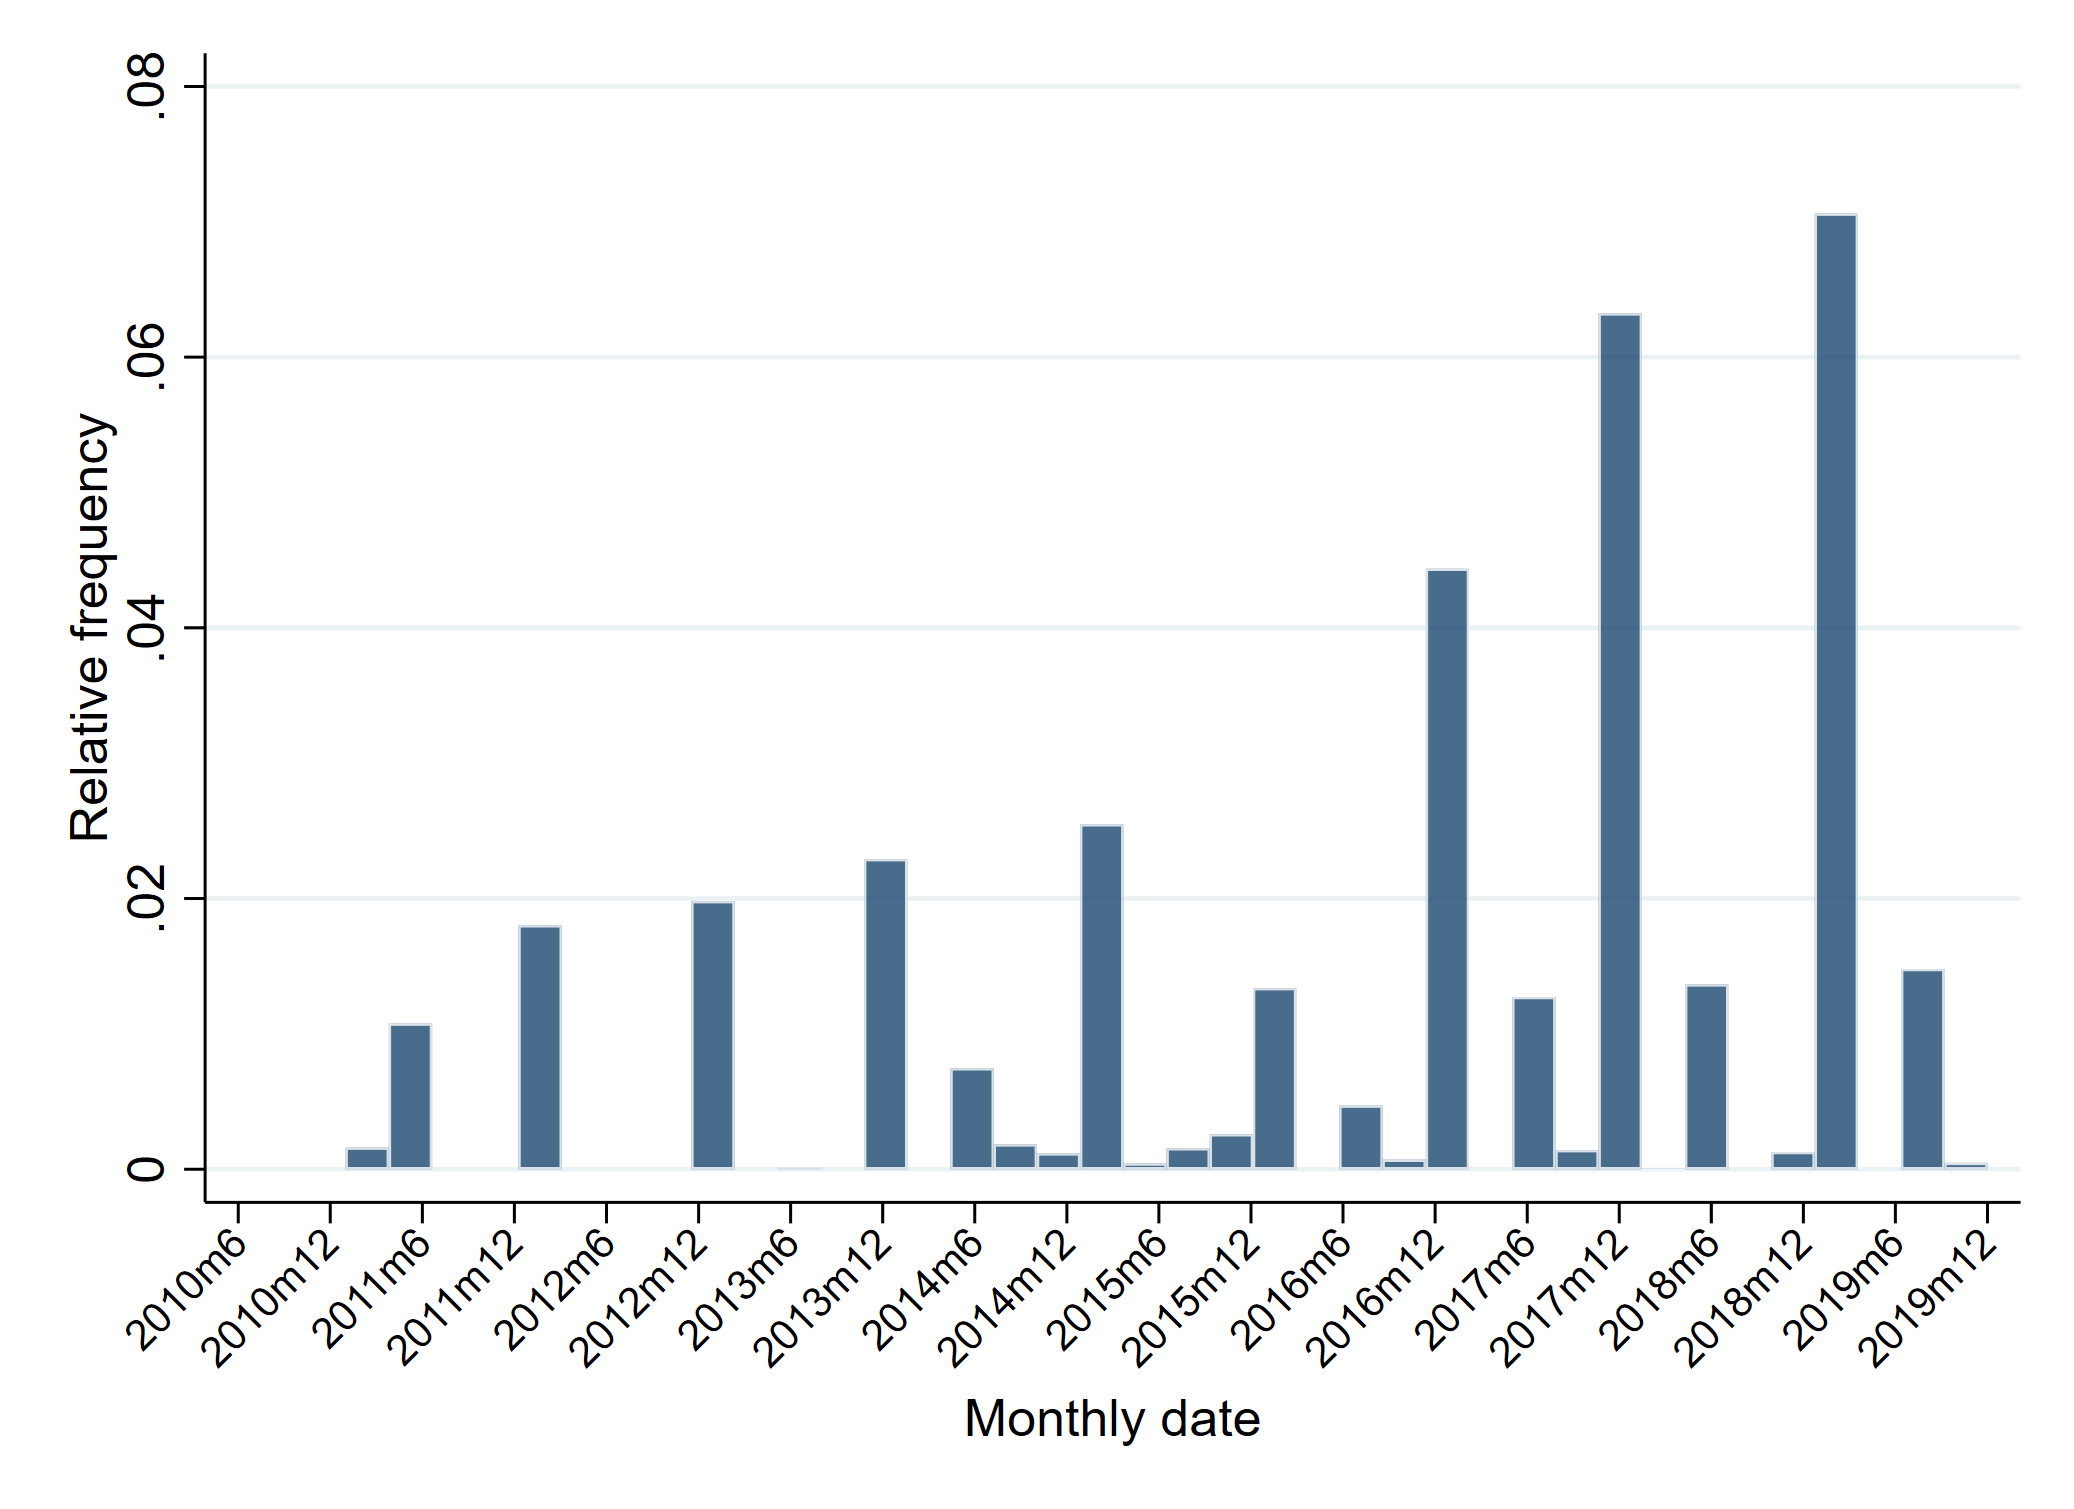
\includegraphics[width = 1\textwidth]
            {estimation_samples/output/pct_ch_mw_date_dist}
    \end{subfigure}

    \begin{minipage}{.95\textwidth} \footnotesize
        \vspace{3mm}
        Notes:
        Data are from the MW panel described in
        Section \ref{sec:data_mw_panel}.
        The histograms show the distribution of positive MW changes in the 
        sample of ZIP codes available in the Zillow data.
        We exclude a few negative changes for expository purposes.
        The top figure (``Intensity'') reports the intensity of the changes in 
        percentage terms.
        The bottom figure (``Timing'') reports the distribution of such changes 
        over time.
    \end{minipage}
\end{figure}
